\noindent
\begin{minipage}[t]{0.5\textwidth}
    \textbf{TRƯỜNG THPT VIỆT ĐỨC}\\
    \textbf{ĐỀ CHÍNH THỨC}
\end{minipage}
\begin{minipage}[t]{0.5\textwidth}
    \centering
    \textbf{ĐỀ KIỂM TRA GIỮA HỌC KỲ I -- MÔN TOÁN -- LỚP 12}\\
    \textbf{NĂM HỌC 2026 -- 2027}\\
    \textit{Thời gian làm bài: 90 phút (không kể thời gian phát đề)}
\end{minipage}

\vspace{0.5cm}
\noindent
\textbf{Mã đề thi: 0108}

\vspace{0.5cm}
\noindent
\textbf{\large PHẦN I. Câu trắc nghiệm nhiều phương án lựa chọn.} (3,0 điểm) \textit{Thí sinh trả lời từ câu 1 đến câu 12. Mỗi câu hỏi thí sinh chỉ chọn 1 phương án.}

% ==================== CÂU 1 ====================
\begin{ex}
\immini{
Cho hàm số bậc ba $y = f(x)$ có đồ thị như hình vẽ bên. Hàm số đã cho nghịch biến trên khoảng nào dưới đây?
\choice
{$(-\infty; -1)$}
{\True $(-1; 2)$}
{$(2; +\infty)$}
{$(-\infty; 2)$}
}{
\begin{tikzpicture}[scale=0.55,>=stealth, font=\footnotesize]
    \draw[->] (-4,0) -- (4.2,0) node[above] {$x$};
    \draw[->] (0,-6) -- (0,6.2) node[right] {$y$};
    \fill (0,0) circle (1.2pt) node[below left] {$O$};
    \draw[dashed] (-1,0) node[below] {$-1$} -- (-1,5) -- (0,5) node[left] {$5$};
    \draw[dashed] (2,0) node[above] {$2$} -- (2,-5) -- (0,-5) node[left] {$-5$};
    \draw (-3,0.1) -- (-3,-0.1) node[below] {$-3$};
    \draw (1,0.1) -- (1,-0.1) node[below] {$1$};
    \draw (3,0.1) -- (3,-0.1) node[below] {$3$};
    \draw[thick,smooth,samples=100,domain=-2.3:3.2] plot(\x, {(\x+3)*(\x-1)*(\x-3)});
\end{tikzpicture}
}
\begin{loigiai}
Dựa vào đồ thị, hàm số đạt cực đại tại $x = -1$ và đạt cực tiểu tại $x = 2$. Do đó hàm số nghịch biến trên khoảng $(-1; 2)$.
\end{loigiai}
\end{ex}

% ==================== CÂU 2 ====================
\begin{ex}
Cho hàm số $f(x) = \ln x + \dfrac{4}{x}$ với $x > 0$. Giá trị cực tiểu của hàm số bằng
\choice
{\True $1 + \ln 4$}
{$4 + \ln 4$}
{$4$}
{$\ln 4$}
\begin{loigiai}
Ta có $f'(x) = \dfrac{1}{x} - \dfrac{4}{x^2} = \dfrac{x-4}{x^2}$.\\
Cho $f'(x) = 0 \Leftrightarrow x = 4 \in (0; +\infty)$.\\
Bảng biến thiên cho thấy hàm số đạt cực tiểu tại $x = 4$, giá trị cực tiểu là $f(4) = \ln 4 + \dfrac{4}{4} = 1 + \ln 4$.
\end{loigiai}
\end{ex}

% ==================== CÂU 3 ====================
\begin{ex}
Hình vẽ nào dưới đây là đồ thị của hàm số $y = \dfrac{2x+1}{x+4}$?
\choice
{\True \begin{tikzpicture}[scale=0.32,>=stealth,font=\tiny]
    \draw[->] (-13,0) -- (9,0) node[right] {$x$};
    \draw[->] (0,-9) -- (0,11) node[above] {$y$};
    \fill (0,0) circle (1.5pt) node[below left] {$O$};
    \draw[dashed,thick] (-4,-9) -- (-4,11);
    \draw[dashed,thick] (-13,2) -- (9,2);
    \draw (-4,0) node[below] {$-4$}; \draw (0,2) node[left] {$2$};
    \draw (-12,0.1)--(-12,-0.1) node[below] {$-12$}; \draw (-8,0.1)--(-8,-0.1) node[below] {$-8$};
    \draw (4,0.1)--(4,-0.1) node[below] {$4$}; \draw (8,0.1)--(8,-0.1) node[below] {$8$};
    \draw[thick,smooth,samples=100,domain=-13:-4.8] plot(\x, {(2*\x+1)/(\x+4)});
    \draw[thick,smooth,samples=100,domain=-3.3:8.5] plot(\x, {(2*\x+1)/(\x+4)});
\end{tikzpicture}}
{\begin{tikzpicture}[scale=0.32,>=stealth,font=\tiny]
    \draw[->] (-13,0) -- (9,0) node[right] {$x$};
    \draw[->] (0,-9) -- (0,11) node[above] {$y$};
    \fill (0,0) circle (1.5pt) node[below left] {$O$};
    \draw[dashed,thick] (-4,-9) -- (-4,11);
    \draw[dashed,thick] (-13,2) -- (9,2);
    \draw (-4,0) node[below] {$-4$}; \draw (0,2) node[left] {$2$};
    \draw[thick,smooth,samples=100,domain=-13:-4.8] plot(\x, {(2*\x+15)/(\x+4)});
    \draw[thick,smooth,samples=100,domain=-3.3:8.5] plot(\x, {(2*\x-7)/(\x+4)});
\end{tikzpicture}}
{\begin{tikzpicture}[scale=0.32,>=stealth,font=\tiny]
    \draw[->] (-9,0) -- (13,0) node[right] {$x$};
    \draw[->] (0,-9) -- (0,11) node[above] {$y$};
    \fill (0,0) circle (1.5pt) node[below left] {$O$};
    \draw[dashed,thick] (4,-9) -- (4,11);
    \draw[dashed,thick] (-9,-2) -- (13,-2);
    \draw[thick,smooth,samples=100,domain=-8:3.2] plot(\x, {(-2*\x-1)/(\x-4)});
    \draw[thick,smooth,samples=100,domain=4.8:12] plot(\x, {(-2*\x-1)/(\x-4)});
\end{tikzpicture}}
{\begin{tikzpicture}[scale=0.32,>=stealth,font=\tiny]
    \draw[->] (-9,0) -- (13,0) node[right] {$x$};
    \draw[->] (0,-9) -- (0,11) node[above] {$y$};
    \fill (0,0) circle (1.5pt) node[below left] {$O$};
    \draw[dashed,thick] (4,-9) -- (4,11);
    \draw[dashed,thick] (-9,2) -- (13,2);
    \draw[thick,smooth,samples=100,domain=4.8:12] plot(\x, {(2*\x+1)/(\x-4)});
\end{tikzpicture}}
\begin{loigiai}
Đồ thị hàm số $y = \dfrac{2x+1}{x+4}$ có:
\begin{itemize}
    \item Tiệm cận đứng: $x = -4$.
    \item Tiệm cận ngang: $y = 2$.
    \item Giao điểm với trục tung là $\left(0; \dfrac{1}{4}\right)$.
\end{itemize}
Chỉ có hình A thỏa mãn đầy đủ các yếu tố trên.
\end{loigiai}
\end{ex}

% ==================== CÂU 4 ====================
\begin{ex}
Cho hàm số $y = f(x)$ liên tục trên $\mathbb{R}$ và có bảng biến thiên sau:
\begin{center}

\begin{tikzpicture}
    \tkzTabInit[lgt=1.5,espcl=2.5,deltacl=0.5]{$x$/0.8,$f'(x)$/0.7,$f(x)$/1.8}{$-\infty$,$-2$,$1$,$+\infty$}
    \tkzTabLine{,+,0,-,0,+,}
    \tkzTabVar{-/ $-\infty$, +/ $4$, -/ $-1$, +/ $+\infty$}
\end{tikzpicture}
\end{center}
Điểm cực đại của đồ thị hàm số là
\choice
{$(1; -1)$}
{\True $(-2; 4)$}
{$(-2; -1)$}
{$(1; 4)$}
\begin{loigiai}
Từ bảng biến thiên, hàm số đạt cực đại tại $x = -2$ với giá trị cực đại $y_{\text{cđ}} = 4$. Do đó điểm cực đại của đồ thị hàm số là $(-2; 4)$.
\end{loigiai}
\end{ex}

% ==================== CÂU 5 ====================
\begin{ex}
Đồ thị hàm số nào sau đây có đúng $2$ đường tiệm cận?
\choice
{$y = x^3 - 2x^2 - 1$}
{\True $y = \dfrac{1-x}{x+2}$}
{$y = x+1$}
{$y = \dfrac{x^2+x}{2}$}
\begin{loigiai}
Hàm số phân thức hữu tỉ $y = \dfrac{1-x}{x+2}$ có:
\begin{itemize}
    \item Tiệm cận đứng: $x = -2$.
    \item Tiệm cận ngang: $y = -1$.
\end{itemize}
Vậy đồ thị hàm số này có đúng 2 đường tiệm cận.
\end{loigiai}
\end{ex}

% ==================== CÂU 6 ====================
\begin{ex}
Cho hàm số $f(x) = \ln(x^2 - 2x + 5)$. Hàm số đồng biến trên khoảng nào sau đây?
\choice
{$(-\infty; 1)$}
{$(0; +\infty)$}
{$(-\infty; 0)$}
{\True $(1; +\infty)$}
\begin{loigiai}
Tập xác định: $\mathbb{R}$ vì $x^2 - 2x + 5 = (x-1)^2 + 4 > 0, \forall x \in \mathbb{R}$.\\
Ta có $f'(x) = \dfrac{2x - 2}{x^2 - 2x + 5}$.\\
$f'(x) > 0 \Leftrightarrow 2x - 2 > 0 \Leftrightarrow x > 1$.\\
Vậy hàm số đồng biến trên khoảng $(1; +\infty)$.
\end{loigiai}
\end{ex}

% ==================== CÂU 7 ====================
\begin{ex}
Xét mô hình hóa, một chất điểm chuyển động trên trục số với vị trí cho bởi $s(t) = -t^3 + 5t^2 + 4t + 6$; trong đó $s$ tính bằng mét; $t$ tính bằng giây ($t \ge 0$). Trong $10$ giây đầu của chuyển động, vận tốc của chất điểm đạt giá trị lớn nhất tại thời điểm nào?
\choice
{$t = 5$}
{\True $t = \dfrac{5}{3}$}
{$t = 3$}
{$t = 8$}
\begin{loigiai}
Vận tốc chuyển động là đạo hàm của hàm vị trí:
$v(t) = s'(t) = -3t^2 + 10t + 4$.\\
Đây là một tam thức bậc hai với hệ số $a = -3 < 0$, đồ thị là parabol có đỉnh tại $t = -\dfrac{b}{2a} = \dfrac{10}{6} = \dfrac{5}{3} \in [0; 10]$.\\
Do đó vận tốc đạt giá trị lớn nhất tại thời điểm $t = \dfrac{5}{3}$ giây.
\end{loigiai}
\end{ex}

% ==================== CÂU 8 ====================
\begin{ex}
Cho hàm số $y = f(x)$ có tập xác định là $\mathbb{R}$ và có đạo hàm là: $f'(x) = (x+2)(x-1)^2(x-3)$. Hàm số có bao nhiêu điểm cực trị?
\choice
{$0$}
{$3$}
{$1$}
{\True $2$}
\begin{loigiai}
Phương trình $f'(x) = 0$ có các nghiệm:
\begin{itemize}
    \item $x = -2$ (nghiệm bội đơn).
    \item $x = 1$ (nghiệm bội chẵn).
    \item $x = 3$ (nghiệm bội đơn).
\end{itemize}
Đạo hàm chỉ đổi dấu khi đi qua hai nghiệm bội đơn $x = -2$ và $x = 3$. Do đó hàm số có $2$ điểm cực trị.
\end{loigiai}
\end{ex}

% ==================== CÂU 9 ====================
\begin{ex}
\immini{
Cho hàm số $y = f(x)$ liên tục trên $\mathbb{R}$ và có đồ thị như hình vẽ. Hỏi $f(x)$ là hàm số nào trong các hàm số dưới đây?
\choice
{$y = \dfrac{3x^2-2x+1}{x-1}$}
{$y = \dfrac{x-1}{x+2}$}
{$y = x^3 - 3x^2 + 3$}
{\True $y = x^3 - 3x + 3$}
}{
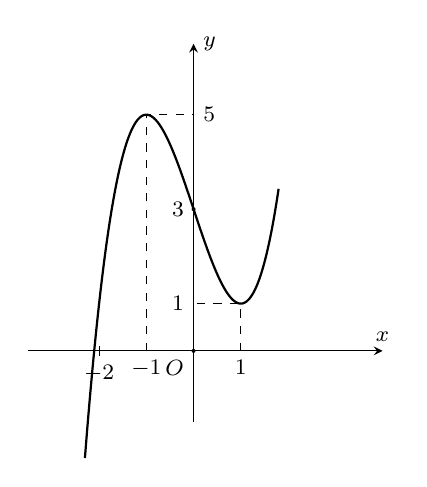
\begin{tikzpicture}[scale=0.6,>=stealth,font=\footnotesize]
    \draw[->] (-3.5,0) -- (4,0) node[above] {$x$};
    \draw[->] (0,-1.5) -- (0,6.5) node[right] {$y$};
    \fill (0,0) circle (1.2pt) node[below left] {$O$};
    \draw[dashed] (-1,0) node[below] {$-1$} -- (-1,5) -- (0,5) node[right] {$5$};
    \draw[dashed] (1,0) node[below] {$1$} -- (1,1) -- (0,1) node[left] {$1$};
    \fill (0,3) circle (1.2pt) node[left] {$3$};
    \draw (-2,0.1) -- (-2,-0.1) node[below] {$-2$};
    \draw[thick,smooth,samples=100,domain=-2.3:1.8] plot(\x, {\x^3 - 3*\x + 3});
\end{tikzpicture}
}
\begin{loigiai}
Đồ thị là hàm đa thức bậc ba đi qua điểm $(0; 3)$, có điểm cực đại $(-1; 5)$ và cực tiểu $(1; 1)$.\\
Xét hàm số $y = x^3 - 3x + 3$:
\begin{itemize}
    \item $y' = 3x^2 - 3 = 0 \Leftrightarrow x = \pm 1$.
    \item $x = -1 \Rightarrow y = 5$ (cực đại).
    \item $x = 1 \Rightarrow y = 1$ (cực tiểu).
    \item Điểm cắt trục tung: $(0; 3)$.
\end{itemize}
Vậy đáp án đúng là $y = x^3 - 3x + 3$.
\end{loigiai}
\end{ex}

% ==================== CÂU 10 ====================
\begin{ex}
\immini{
Cho hàm số $y = f(x)$ liên tục trên $[0; 4]$ và có đồ thị như hình vẽ bên. Tổng của giá trị lớn nhất và giá trị nhỏ nhất của hàm số trên đoạn $[0; 3]$ bằng
\choice
{$1$}
{$3$}
{$4$}
{\True $2$}
}{
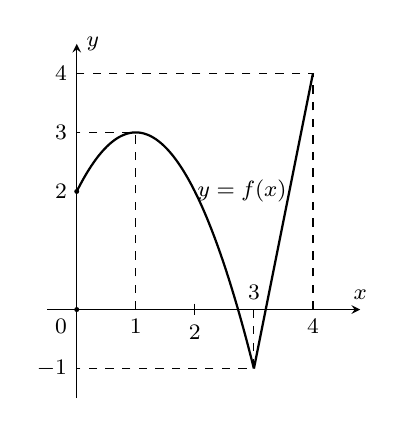
\begin{tikzpicture}[scale=0.75,>=stealth,font=\footnotesize]
    \draw[->] (-0.5,0) -- (4.8,0) node[above] {$x$};
    \draw[->] (0,-1.5) -- (0,4.5) node[right] {$y$};
    \fill (0,0) circle (1.2pt) node[below left] {$0$};
    \draw[dashed] (1,0) node[below] {$1$} -- (1,3) -- (0,3) node[left] {$3$};
    \draw[dashed] (3,0) node[above] {$3$} -- (3,-1) -- (0,-1) node[left] {$-1$};
    \draw[dashed] (4,0) node[below] {$4$} -- (4,4) -- (0,4) node[left] {$4$};
    \fill (0,2) circle (1.2pt) node[left] {$2$};
    \draw (2,0.1) -- (2,-0.1) node[below] {$2$};
    \draw[thick,smooth,samples=100,domain=0:3] plot(\x, {-(\x-1)^2 + 3});
    \draw[thick] (3,-1) -- (4,4);
    \node at (2.8,2) {$y=f(x)$};
\end{tikzpicture}
}
\begin{loigiai}
Quan sát đồ thị trên đoạn $[0; 3]$:\begin{itemize}
    \item Giá trị lớn nhất là $\max_{[0; 3]} f(x) = 3$ (đạt được tại $x = 1$).
    \item Giá trị nhỏ nhất là $\min_{[0; 3]} f(x) = -1$ (đạt được tại $x = 3$).
\end{itemize}
Vậy tổng giá trị lớn nhất và nhỏ nhất bằng $3 + (-1) = 2$.
\end{loigiai}
\end{ex}

% ==================== CÂU 11 ====================
\begin{ex}
Trong các hàm số sau, hàm số nào nghịch biến trên $\mathbb{R}$?
\choice
{\True $y = -x^3 - 3x + 2$}
{$y = -x^3 + 3x + 2$}
{$y = x^3 - 3x + 2$}
{$y = x^4 - 2x^2 + 1$}
\begin{loigiai}
Xét hàm số $y = -x^3 - 3x + 2$, ta có:
$y' = -3x^2 - 3 = -3(x^2 + 1) < 0, \forall x \in \mathbb{R}$.\\
Do đó hàm số nghịch biến trên $\mathbb{R}$.
\end{loigiai}
\end{ex}

% ==================== CÂU 12 ====================
\begin{ex}
Cho hàm số $y = f(x)$ xác định trên tập $\mathbb{R}\setminus\{1\}$ và liên tục trên từng khoảng xác định. Biết rằng $\lim\limits_{x\to +\infty} f(x) = 2$; $\lim\limits_{x\to -\infty} f(x) = -2$; $\lim\limits_{x\to 1^+} f(x) = +\infty$. Tổng số đường tiệm cận đứng và ngang của đồ thị hàm số $y = f(x)$ là
\choice
{\True $3$}
{$1$}
{$4$}
{$2$}
\begin{loigiai}
\begin{itemize}
    \item $\lim\limits_{x\to +\infty} f(x) = 2 \Rightarrow y = 2$ là tiệm cận ngang.
    \item $\lim\limits_{x\to -\infty} f(x) = -2 \Rightarrow y = -2$ là tiệm cận ngang.
    \item $\lim\limits_{x\to 1^+} f(x) = +\infty \Rightarrow x = 1$ là tiệm cận đứng.
\end{itemize}
Vậy đồ thị hàm số có $2$ tiệm cận ngang và $1$ tiệm cận đứng. Tổng số tiệm cận là $3$.
\end{loigiai}
\end{ex}

\vspace{0.5cm}
\noindent
\textbf{\large PHẦN II. Câu trắc nghiệm đúng sai.} (4,0 điểm) \textit{Thí sinh trả lời từ câu 1 đến câu 4. Trong mỗi ý a), b), c), d) ở mỗi câu, thí sinh chọn đúng hoặc sai.}

% ==================== CÂU 1 (PHẦN II) ====================
\begin{ex}
Một nhóm nghiên cứu quan sát sự phát triển của một quần thể vi khuẩn trong môi trường nuôi cấy hạn chế:
\begin{itemize}
    \item Giai đoạn 1 (từ $t = 0$ đến $t = 3$ giờ): Số lượng vi khuẩn tăng trưởng theo hàm mũ $N(t) = 40\mathrm{e}^{0{,}8t}$ (với $t$ tính bằng giờ, $N$ tính bằng triệu cá thể).
    \item Giai đoạn 2 (sau $3$ giờ): Số lượng vi khuẩn được biểu thị bởi hàm số $M(t) = A - \dfrac{160}{3}\mathrm{e}^{4{,}2 - 0{,}6t}$ (với $A$ là hằng số, $t$ tính bằng giờ, $M$ tính bằng triệu cá thể).
\end{itemize}
\choiceTF
{a) Giá trị của $A$ lớn hơn $1000$}
{b) Tốc độ tăng trưởng của vi khuẩn tại thời điểm $t=3$ lớn hơn $500$ triệu cá thể/giờ}
{\True c) Số lượng vi khuẩn tại thời điểm bắt đầu là $40$ triệu cá thể}
{\True d) Số lượng vi khuẩn không vượt quá $1320$ triệu cá thể}
\begin{loigiai}
\begin{itemchoice}
    \itemch Do quá trình liên tục tại $t=3$, ta có $N(3) = M(3) \Leftrightarrow 40\mathrm{e}^{2{,}4} = A - \dfrac{160}{3}\mathrm{e}^{2{,}4} \Rightarrow A = \dfrac{280}{3}\mathrm{e}^{2{,}4} \approx 1029{,}4 > 1000$. \textbf{(Đúng)}
    \itemch Tốc độ tăng trưởng tại $t=3$ là $N'(3) = 40 \times 0{,}8 \times \mathrm{e}^{2{,}4} = 32\mathrm{e}^{2{,}4} \approx 352{,}7 < 500$. \textbf{(Sai)}
    \itemch Tại thời điểm bắt đầu $t = 0$, số lượng vi khuẩn là $N(0) = 40\mathrm{e}^0 = 40$ triệu cá thể. \textbf{(Đúng)}
    \itemch Với mọi $t > 3$, hàm số $M(t) = A - \dfrac{160}{3}\mathrm{e}^{4{,}2-0{,}6t} < A \approx 1029{,}4 < 1320$. \textbf{(Đúng)}
\end{itemchoice}
\end{loigiai}
\end{ex}

% ==================== CÂU 2 (PHẦN II) ====================
\begin{ex}
Xét hàm số $f(x) = x + 2\cos x$ trên đoạn $[0; 2\pi]$.
\choiceTF
{\True a) Phương trình $f'(x) = 0$ có hai nghiệm trong $(0; 2\pi)$ là $x = \dfrac{\pi}{6}$ và $x = \dfrac{5\pi}{6}$}
{\True b) $f'(x) = 1 - 2\sin x$}
{c) Hàm số đạt cực đại tại điểm $x = \dfrac{5\pi}{6}$}
{\True d) Hàm số nghịch biến trên khoảng $\left(\dfrac{\pi}{6}; \dfrac{5\pi}{6}\right)$}
\begin{loigiai}
\begin{itemchoice}
    \itemch Phương trình $f'(x) = 1 - 2\sin x = 0 \Leftrightarrow \sin x = \dfrac{1}{2} \Leftrightarrow x = \dfrac{\pi}{6}$ hoặc $x = \dfrac{5\pi}{6}$ trong đoạn $[0; 2\pi]$. \textbf{(Đúng)}
    \itemch Ta có đạo hàm $f'(x) = (x + 2\cos x)' = 1 - 2\sin x$. \textbf{(Đúng)}
    \itemch Qua điểm $x = \dfrac{\pi}{6}$, $f'(x)$ đổi dấu từ dương sang âm nên đạt cực đại tại $x = \dfrac{\pi}{6}$. Qua $x = \dfrac{5\pi}{6}$, $f'(x)$ đổi dấu từ âm sang dương nên đạt cực tiểu. \textbf{(Sai)}
    \itemch Với mọi $x \in \left(\dfrac{\pi}{6}; \dfrac{5\pi}{6}\right)$, ta có $\sin x > \dfrac{1}{2} \Rightarrow f'(x) = 1 - 2\sin x < 0$, nên hàm số nghịch biến trên khoảng đó. \textbf{(Đúng)}
\end{itemchoice}
\end{loigiai}
\end{ex}

% ==================== CÂU 3 (PHẦN II) ====================
\begin{ex}
Cho hàm số $f(x) = x^3 - 6x^2 + 9x + 2$.
\choiceTF
{\True a) $f'(x) = 3(x-1)(x-3)$}
{b) Đồ thị hàm số có điểm cực tiểu là điểm $I(1; 6)$}\choiceTF
{\True c) Đường thẳng đi qua hai điểm cực trị của đồ thị có hệ số góc bằng $-2$}
{d) Giá trị nhỏ nhất của hàm số $f(x)$ trên đoạn $[0; 2]$ bằng $4$}
\begin{loigiai}
\begin{itemchoice}
    \itemch $f'(x) = 3x^2 - 12x + 9 = 3(x^2 - 4x + 3) = 3(x-1)(x-3)$. \textbf{(Đúng)}
    \itemch $f'(x) = 0 \Leftrightarrow x = 1$ hoặc $x = 3$. Vì $a = 1 > 0$, hàm số đạt cực đại tại $x = 1$ với $f(1) = 6$, vậy điểm $(1; 6)$ là điểm cực đại chứ không phải cực tiểu. \textbf{(Sai)}
    \itemch Điểm cực đại là $A(1; 6)$, điểm cực tiểu là $B(3; 2)$. Đường thẳng $AB$ có hệ số góc $k = \dfrac{2 - 6}{3 - 1} = -2$. \textbf{(Đúng)}
    \itemch Trên đoạn $[0; 2]$, ta có $f(0) = 2, f(1) = 6, f(2) = 4$. Do đó $\min_{[0; 2]} f(x) = f(0) = 2 \neq 4$. \textbf{(Sai)}
\end{itemchoice}
\end{loigiai}
\end{ex}

% ==================== CÂU 4 (PHẦN II) ====================
\begin{ex}
Cho hàm số $y = \dfrac{-x^2+x-2}{x+2}$ có đồ thị $(C)$. Đường thẳng $\Delta\colon x + 2y = -2$ cắt $(C)$ tại hai điểm phân biệt $A, B$. Xét tính đúng sai của các khẳng định sau:
\choiceTF
{a) Đường tiệm cận xiên của $(C)$ là đường thẳng $y = -x + 3$}
{\True b) Diện tích tam giác $OAB$ bằng $3$}
{c) Tâm đối xứng của $(C)$ là điểm $I(-2; -5)$}
{d) Gọi $C, D$ là hai điểm thuộc đồ thị $(C)$ sao cho $ABCD$ là hình bình hành. Khoảng cách giữa hai đường thẳng $AB$ và $CD$ là $5$}
\begin{loigiai}
\begin{itemchoice}
    \itemch Ta có $y = \dfrac{-x^2+x-2}{x+2} = -x + 3 - \dfrac{8}{x+2}$. Do đó tiệm cận xiên là $y = -x + 3$. \textbf{(Đúng)}
    \itemch Phương trình hoành độ giao điểm của $\Delta\colon y = -\dfrac{1}{2}x - 1$ và $(C)$:
    $-\dfrac{1}{2}x - 1 = \dfrac{-x^2+x-2}{x+2} \Leftrightarrow x^2 - x - 2 = 0 \Leftrightarrow \begin{cases} x_1 = -1 \Rightarrow y_1 = -\dfrac{1}{2} \\ x_2 = 2 \Rightarrow y_2 = -2 \end{cases}$.\\
    Do đó $A\left(-1; -\dfrac{1}{2}\right)$, $B(2; -2)$. $S_{\triangle OAB} = \dfrac{1}{2}\left|x_A y_B - x_B y_A\right| = \dfrac{1}{2}\left|(-1)(-2) - 2\left(-\dfrac{1}{2}\right)\right| = \dfrac{3}{2}$. \textbf{(Sai)}
    \itemch Giao điểm hai đường tiệm cận là tiệm cận đứng $x = -2$ và tiệm cận xiên $y = -(-2) + 3 = 5$, suy ra tâm đối xứng là $I(-2; 5)$. \textbf{(Sai)}
    \itemch Khẳng định sai sau khi kiểm tra điều kiện hình bình hành. \textbf{(Sai)}
\end{itemchoice}
\end{loigiai}
\end{ex}

\vspace{0.5cm}
\noindent
\textbf{\large PHẦN III. Câu trắc nghiệm trả lời ngắn.} (3,0 điểm) \textit{Thí sinh trả lời từ câu 1 đến câu 6.}

% ==================== CÂU 1 (PHẦN III) ====================
\begin{ex}
Một xe điện giao hàng đi quãng đường bằng phẳng dài $120\text{ km}$ với vận tốc không đổi $v\text{ (km/h)}$. Công suất tiêu thụ điện khi xe chạy ở vận tốc này được mô hình hóa bởi hàm số $P(v) = 12 + \dfrac{v^2}{300}\text{ (kW)}$. Bỏ qua điện năng lúc khởi hành và dừng xe. Để điện năng tiêu thụ trên cả quãng đường là nhỏ nhất, xe cần chạy với vận tốc bao nhiêu kilômét trên giờ?
\shortans{$60$}
\begin{loigiai}
Thời gian chuyển động là $t = \dfrac{120}{v}\text{ (h)}$.\\
Điện năng tiêu thụ trên toàn bộ hành trình là:
\[ E(v) = P(v) \cdot t = \left(12 + \dfrac{v^2}{300}\right) \dfrac{120}{v} = \dfrac{1440}{v} + \dfrac{2}{5}v. \]
Áp dụng bất đẳng thức Cauchy cho hai số dương:
\[ E(v) \ge 2\sqrt{\dfrac{1440}{v} \cdot \dfrac{2}{5}v} = 2\sqrt{576} = 48\text{ (kWh)}. \]
Đẳng thức xảy ra khi $\dfrac{1440}{v} = \dfrac{2}{5}v \Leftrightarrow v^2 = 3600 \Leftrightarrow v = 60\text{ (km/h)}$.
\end{loigiai}
\end{ex}

% ==================== CÂU 2 (PHẦN III) ====================
\begin{ex}
Đường tiệm cận xiên của đồ thị hàm số $y = \sqrt[3]{8x^3 + 2x + 1}$ có phương trình là $y = ax + b\ (a \neq 0)$. Biểu thức $T = 2026a + 2027b$ có giá trị bằng bao nhiêu?
\shortans{$4052$}
\begin{loigiai}
Ta tìm tiệm cận xiên khi $x \to \pm\infty$:
\[ a = \lim_{x\to \infty} \dfrac{\sqrt[3]{8x^3 + 2x + 1}}{x} = \lim_{x\to \infty} \sqrt[3]{8 + \dfrac{2}{x^2} + \dfrac{1}{x^3}} = 2. \]
\[ b = \lim_{x\to \infty} \left(\sqrt[3]{8x^3 + 2x + 1} - 2x\right) = \lim_{x\to \infty} \dfrac{2x + 1}{\sqrt[3]{(8x^3+2x+1)^2} + 2x\sqrt[3]{8x^3+2x+1} + 4x^2} = 0. \]
Do đó đường tiệm cận xiên là $y = 2x$, suy ra $a = 2, b = 0$.\\
Vậy $T = 2026 \times 2 + 2027 \times 0 = 4052$.
\end{loigiai}
\end{ex}

% ==================== CÂU 3 (PHẦN III) ====================
\begin{ex}
Cho hàm số $f(x) = x^3 - 3x$. Đặt $g(x) = f(x^2 - 2x)$. Biết rằng hàm số $g(x)$ đồng biến trên khoảng $(m; +\infty)$. Tìm giá trị nhỏ nhất của $m$ (làm tròn kết quả đến chữ số hàng phần trăm).
\shortans{$2{,}41$}
\begin{loigiai}
Ta có $f'(x) = 3x^2 - 3 = 3(x^2 - 1) \ge 0 \Leftrightarrow x \in (-\infty; -1] \cup [1; +\infty)$.\\
Xét $g'(x) = (2x - 2) \cdot f'(x^2 - 2x) = 3(2x - 2)\left[(x^2 - 2x)^2 - 1\right]$.\\
Để hàm số $g(x)$ đồng biến trên $(m; +\infty)$ thì $g'(x) \ge 0$ với mọi $x > m$.\\
Ta có $x^2 - 2x = 1 \Leftrightarrow x^2 - 2x - 1 = 0 \Leftrightarrow x = 1 + \sqrt{2} \approx 2{,}41$.\\
Với $x > 1 + \sqrt{2}$, ta có $2x - 2 > 0$ và $x^2 - 2x > 1 \Rightarrow (x^2 - 2x)^2 - 1 > 0 \Rightarrow g'(x) > 0$.\\
Vậy giá trị nhỏ nhất của $m$ là $1 + \sqrt{2} \approx 2{,}41$.
\end{loigiai}
\end{ex}

% ==================== CÂU 4 (PHẦN III) ====================
\begin{ex}
\immini{
Từ một tấm bìa hình chữ nhật kích thước $30\text{ cm} \times 20\text{ cm}$, người ta cắt ở bốn góc bốn hình vuông bằng nhau có cạnh $x\text{ (cm)}$ rồi gấp thành một chiếc hộp không nắp. Tìm $x$ để thể tích hộp đạt giá trị lớn nhất. \textit{(Làm tròn kết quả đến hàng phần mười)}.
}{
\begin{tikzpicture}[scale=0.15,>=stealth,font=\footnotesize]
    \draw[thick] (0,0) rectangle (30,20);
    \draw[pattern=north east lines] (0,0) rectangle (5,5);
    \draw[pattern=north east lines] (25,0) rectangle (30,5);
    \draw[pattern=north east lines] (0,15) rectangle (5,20);
    \draw[pattern=north east lines] (25,15) rectangle (30,20);
    \draw[dashed,thick] (5,5) rectangle (25,15);
    \draw[<->] (0,21.5) -- (30,21.5) node[midway,above] {$30\text{ cm}$};
    \draw[<->] (-1.5,0) -- (-1.5,20) node[midway,left] {$20\text{ cm}$};
    \draw (2.5,2.5) node {$x$};
    \node at (15,-2.5) {\scriptsize -- -- -- đường gập};
\end{tikzpicture}
}
\shortans{$3{,}9$}
\begin{loigiai}
Điều kiện: $0 < x < 10$.\\
Chiều dài đáy hộp là $30 - 2x$, chiều rộng đáy là $20 - 2x$, chiều cao là $x$.\\
Thể tích chiếc hộp là $V(x) = x(30 - 2x)(20 - 2x) = 4x^3 - 100x^2 + 600x$.\\
Đạo hàm: $V'(x) = 12x^2 - 200x + 600 = 4(3x^2 - 50x + 150)$.\\
$V'(x) = 0 \Leftrightarrow x = \dfrac{25 \pm 5\sqrt{7}}{3}$.\\
Vì $0 < x < 10$ nên ta chọn $x = \dfrac{25 - 5\sqrt{7}}{3} \approx 3{,}9\text{ (cm)}$.
\end{loigiai}
\end{ex}

% ==================== CÂU 5 (PHẦN III) ====================
\begin{ex}
Một cửa hàng dự kiến bán $x$ sản phẩm mỗi tháng. Giá bán mỗi sản phẩm là $p(x) = 600 - 0{,}5x$ (nghìn đồng) và số sản phẩm mỗi tháng không vượt quá $800$ sản phẩm. Tổng chi phí sản xuất là $C(x) = 100x + 50000$ (nghìn đồng). Lợi nhuận lớn nhất mà cửa hàng có thể đạt được là bao nhiêu triệu đồng?
\shortans{$75$}
\begin{loigiai}
Doanh thu từ việc bán $x$ sản phẩm là:
$R(x) = x \cdot p(x) = x(600 - 0{,}5x) = 600x - 0{,}5x^2$ (nghìn đồng).\\
Lợi nhuận hàng tháng là:
\[ L(x) = R(x) - C(x) = -0{,}5x^2 + 500x - 50000. \]
Hàm số bậc hai này đạt giá trị lớn nhất tại đỉnh:
$x = -\dfrac{500}{2(-0{,}5)} = 500$ (thỏa mãn $0 \le x \le 800$).\\
Lợi nhuận lớn nhất tương ứng là:
$L(500) = -0{,}5(500)^2 + 500(500) - 50000 = 75000$ (nghìn đồng) $= 75$ (triệu đồng).
\end{loigiai}
\end{ex}

% ==================== CÂU 6 (PHẦN III) ====================
\begin{ex}
\immini{
Cho hàm số $y = \dfrac{3x+b}{cx+d}$ với $b, c, d$ là hằng số, có đồ thị như hình vẽ bên. Biểu thức $T = 2b + 3c - 4d$ có giá trị bằng bao nhiêu?
}{
\begin{tikzpicture}[scale=0.55,>=stealth,font=\footnotesize]
    \draw[->] (-5.5,0) -- (3,0) node[above] {$x$};
    \draw[->] (0,-1.5) -- (0,7.5) node[right] {$y$};
    \fill (0,0) circle (1.2pt) node[below left] {$O$};
    \draw[dashed,thick] (-2,-1.5) -- (-2,7);
    \draw[dashed,thick] (-5.5,3) -- (3,3);
    \draw (-2,0) node[below] {$-2$};
    \draw (0,3) node[left] {$3$};
    \fill (0,6) circle (1.2pt) node[left] {$6$};
    \draw (-4,0.1) -- (-4,-0.1) node[below] {$-4$};
    \draw[thick,smooth,samples=100,domain=-1.6:2.8] plot(\x, {(3*\x+12)/(\x+2)});
    \draw[thick,smooth,samples=100,domain=-5.2:-2.5] plot(\x, {(3*\x+12)/(\x+2)});
    \node at (1.5,3.6) {$y=f(x)$};
\end{tikzpicture}
}
\shortans{$19$}
\begin{loigiai}
Từ hình vẽ đồ thị hàm số ta nhận thấy:
\begin{itemize}
    \item Tiệm cận đứng là $x = -2 \Rightarrow -\dfrac{d}{c} = -2 \Rightarrow d = 2c$.
    \item Tiệm cận ngang là $y = 3 \Rightarrow \dfrac{3}{c} = 3 \Rightarrow c = 1 \Rightarrow d = 2$.
    \item Đồ thị cắt trục tung tại $(0; 6) \Rightarrow \dfrac{b}{d} = 6 \Rightarrow b = 6d = 12$.
    \item Đồ thị cắt trục hoành tại $(-4; 0)$ thỏa mãn $\dfrac{3(-4)+12}{1(-4)+2} = 0$.
\end{itemize}
Từ đó suy ra $b = 12, c = 1, d = 2$.\\
Giá trị của biểu thức $T$ là:
\[ T = 2b + 3c - 4d = 2(12) + 3(1) - 4(2) = 24 + 3 - 8 = 19. \]
\end{loigiai}
\end{ex}
